\documentclass[a4paper,10pt]{book}
\usepackage{xypic}
\usepackage[centertags]{amsmath}
\usepackage{amscd}
\usepackage{amsthm}
\usepackage{amssymb}
\usepackage{enumerate}
\usepackage{multicol}
\usepackage[english]{babel}
\usepackage[all]{xy}
\usepackage{color}
\usepackage{tikz}
\usepackage{indentfirst}
\usepackage[utf8]{inputenc}
\usepackage[T1]{fontenc}
\linespread{1.1}
\setlength{\parskip}{10pt}
\usepackage[twoside,bindingoffset=1cm]{geometry}
\usepackage{lmodern}


%% Custom packages


%%%%%%%%%%%%%%%%%%%%%%%%%%%%%%%%%%%%%%%%%%%%%%%%%%%%%%%%%%%%%%%%%%%%%%%%%%%
%%%% local definitions for this paper
%%%%%%%%%%%%%%%%%%%%%%%%%%%%%%%%%%%%%%%%%%%%%%%%%%%%%%%%%%%%%%%%%%%%%%%%%%%


%%%%%%%%%%%%%%%%%%%%%% aix{\`o} pels headings %%%%%%%%%%%%%%%%%%%%%%%%
\usepackage{fancyhdr}
\pagestyle{fancy}
\renewcommand{\chaptermark}[1]{\markboth{#1}{}}
\renewcommand{\sectionmark}[1]{\markright{\thesection\ #1}}
\fancyhf{} \fancyhead[LE,RO]{\bfseries\thepage}
\fancyhead[LO]{\bfseries\rightmark} \fancyhead[RE]{\bfseries\leftmark}

\def\paginaenblanc{\newpage%
\thispagestyle{empty}%
\vspace*{2cm}%
\newpage%
\thispagestyle{empty}%
}


%%%%%%%%%%%%%%%%%%%%%%%%%%%%%%%%%%%%%%%%%%%%%%%%%%%%%%%%%%%%%%%%%%%%%%%%%
% aux commands
%%%%%%%%%%%%%%%%%%%%%%%%%%%%%%%%%%%%%%%%%%%%%%%%%%%%%%%%%%%%%%%%%%%%%%%%%
%==========================================================================
% macros to support private authors' notes
%==========================================================================
\newif\ifprivate
\privatetrue
\def\xbar{\vskip0.09in\hrule\vskip0.06in}
\def\private#1{\ifprivate \xbar {\em #1} \xbar
\else \fi}
\def\huh{\ifprivate ??? \marginpar{\Huge ???}
\else \fi}
\def\???{\ifprivate {\bf {???}} \marginpar{\begin{center}{\Huge {\bf ?}}\end{center}}
\else \fi}
%\def\???{\ifprivate {\bf {???}} \marginpar{{\Huge {\bf ?}}}
%\else \fi}
\marginparsep1mm
\def\nota#1{\ifprivate  $\clubsuit$ \marginpar{\parbox[t]{2.4cm}{\begin{center}\tiny #1\end{center}}}
\else \fi}
\def\comment#1{\ifprivate \marginpar{\parbox[t]{2.4cm}{\begin{center}\tiny #1\end{center}}}
\else \fi}
%\def\nota#1{\ifprivate  $\clubsuit$ \marginpar{\parbox[t]{1.8cm}{\tiny #1}}
%\else \fi}
\def\privateeject{\ifprivate\eject\fi}
%\def\???{{\bf {???}} \marginpar{{\Huge {\bf ?}}} }
%%%%%%%%%%%%%%%%%%%%%%%%%%%%%%%%%%%%%%%%%%%%%%%%%%%%%%%%%%%%%%%%%%%%%%%%%%

%%%%%%%%%%%%%%%%%%%%%%%%%%%%%%%%%%%%%%%%%%%%%%%%%%%%%%%%%%%%%%%%%%%%%%%%
%%%%%%%%%%%%%%%%%%%%%%%%%%%%%%%%%%%%%%%%%%%%%%%%%%%%%%%%%%%%%%%%%%%%%%%%
\begin{document}

\pagestyle{empty}

\begin{titlepage}
\begin{center}
\begin{figure}[htb]
\begin{center}

\includegraphics[width=6cm]{assets/ub_color.pdf}
\end{center}
\end{figure}

\def\worktitle{Development of an AI-Based Tool for Molecular Subtype Classification of Invasive Ductal Breast Carcinoma Using Mammography}

\textbf{\LARGE Treball final de grau} \\
\vspace*{.5cm}
\textbf{\LARGE GRAU D'ENGINYERIA INFORM\`{A}TICA } \\
\vspace*{.5cm}
\textbf{\LARGE Facultat de Matem\`atiques i Inform\`atica\\ Universitat de Barcelona} \\
\vspace*{1.0cm}
\rule{16cm}{0.1mm}\\
\begin{Huge}
\textbf{Development of an AI-Based Tool for Molecular Subtype Classification of Invasive Ductal Breast Carcinoma Using Mammography} \\
\end{Huge}
\rule{16cm}{0.1mm}\\

\vspace{1cm}

\begin{flushright}


\vspace*{2.5cm}

\hfill

\renewcommand{\arraystretch}{1.5}
\begin{tabular}{ll}
\textbf{\small Autor:} & \textbf{\small David Bland\'on T\'orrez } \\
\textbf{\small Director:} & \textbf{\small Dr. Oliver D\'iaz Montesdeoca } \\
\textbf{\small Realitzat a:} & \textbf{\small  Departament de Matem\`{a}tiques i  Inform\`{a}tica  } \\
\textbf{\small Barcelona,} & \textbf{\small \today }
\end{tabular}

\end{flushright}

\end{center}

\end{titlepage}

%%%%%%%%%%%%%%%%%%%%%%%%%%%%%%%%%%%%%%%%%%%%%%%%%%%%%%%%%%%%%%%%%%%%%%%%%
\newpage
\selectlanguage{english}
\noindent \textbf{\large Abstract}

// TODO

%%%%%%%%%%%%%%%%%%%%%%%%%%%%%%%%%%%%%%%%%%%%%%%%%%%%%%%%%%%%%%%%%%%%%%%%%

%%%%%%%%%%%%%%%%%%%%%%%%%%%%%%%%%%%%%%%%%%%%%%%%%%%%%%%%%%%%%%%%%%%%%%%%%
\newpage
\selectlanguage{spanish}
\noindent \textbf{\large Resumen}

// TODO

%%%%%%%%%%%%%%%%%%%%%%%%%%%%%%%%%%%%%%%%%%%%%%%%%%%%%%%%%%%%%%%%%%%%%%%%%

%%%%%%%%%%%%%%%%%%%%%%%%%%%%%%%%%%%%%%%%%%%%%%%%%%%%%%%%%%%%%%%%%%%%%%%%%
\newpage
\selectlanguage{catalan}
\noindent \textbf{\large Resum}

// TODO

%%%%%%%%%%%%%%%%%%%%%%%%%%%%%%%%%%%%%%%%%%%%%%%%%%%%%%%%%%%%%%%%%%%%%%%%%
\newpage
\selectlanguage{english}
\noindent \textbf{\large Acknowledgements}

// TODO
%%%%%%%%%%%%%%%%%%%%%%%%%%%%%%%%%%%%%%%%%%%%%%%%%%%%%%%%%%%%%%%%%%%%%%%%%
\selectlanguage{english}
\pagenumbering{roman} \setcounter{page}{0}
\let\cleardoublepage\clearpage
\tableofcontents
\newpage \thispagestyle{empty}
%%%%%%%%%%%%%%%%%%%%%%%%%%%%%%%%%%%%%%%%%%%%%%%%%%%%%%%%%%%%%%%%%%%%%%%%%

\pagestyle{fancy}
\markboth{Introducción}{Introducción}
\newpage \thispagestyle{empty}
%%%%%%%%%%%%%%%%%%%%%%%%%%%%%%%%%%%%%%%%%%%%%%%%%%%%%%%%%%%%%%%%%%%%%%%%%
\mainmatter
\chapter{Introduction}
\section{Problem Context}

In recent years, breast cancer has become one of the leading causes of death among women and represents the most common type of cancer in this population. It is estimated that, on average, one in twenty women worldwide will be diagnosed with this disease during their lifetime \cite{kim_global_2025}. Recent projections suggest that, if current trends continue, by 2050 approximately 3.2 million new cases and 1.1 million deaths associated with this condition will be recorded, with a particularly significant impact in countries with a low Human Development Index (HDI) \cite{kim_global_2025}.

In this context, early diagnostic techniques and tools play a key role in improving patients' prognosis and survival \cite{wang_early_2017}.

However, breast cancer is a heterogeneous disease\footnote{Cellular diversity within a tumor (intratumoral heterogeneity) or between tumors in the same individual (intertumoral heterogeneity).} that can be classified into different subtypes based on clinical and especially molecular characteristics \cite{orrantia-borunda_subtypes_2022}. Therefore, prognosis, therapy response, and treatment options largely depend on the correct identification of the molecular subtype.

Currently, molecular characterization of the tumor is mainly performed via biopsy, an invasive and costly procedure that sometimes needs to be repeated, which can delay treatment initiation and increase patient burden. Thus, there is a growing need to develop non-invasive, accessible, and efficient methods to reliably perform this task.

In this regard, mammography stands out as a key tool, as it is a non-invasive, low-cost, and widely used technique for early breast cancer detection.

With the emergence of artificial intelligence and deep learning techniques, breast cancer detection via mammography has seen significant advances, reaching accuracies comparable to or even exceeding those of expert radiologists \cite{pattanaik_breast_2022, meenalochini_deep_2024, zahoor_breast_2022}. More recently, these methodologies have begun to be applied to the automatic classification of molecular subtypes from mammographic images, opening new possibilities for the development of non-invasive tumor characterization methods \cite{mota_breast_2024, ben_rabah_multimodal_2025}.

... //TODO: Develop conclusion

\begin{figure}
    \centering
    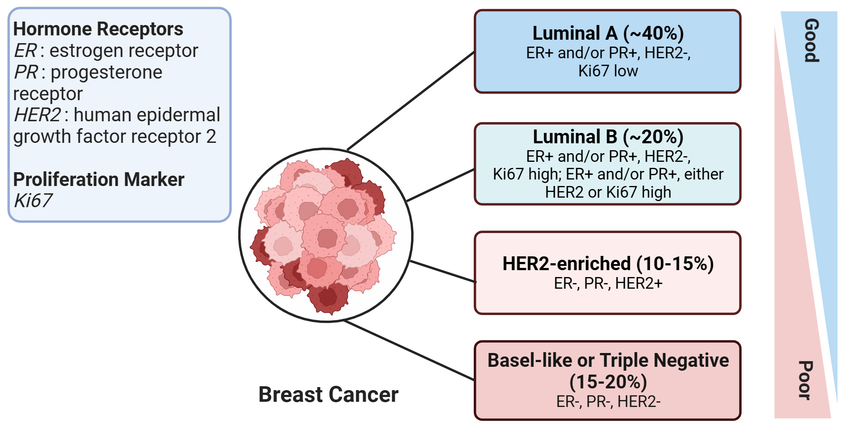
\includegraphics[width=0.8\linewidth]{reports/assets/subtypes.png}
    \caption{The 4 molecular subtypes of breast cancer and their prevalence percentage \cite{harnessing_2024}}
    \label{fig:subtypes}
\end{figure}

\section{Objectives}

The main objective of this study is to develop a deep learning model capable of classifying molecular subtypes of breast cancer using only mammographic images from the \textit{Chinese Mammography Database} (CMMD), without relying on clinical metadata or auxiliary annotations. This task poses significant challenges, such as class imbalance between molecular subtypes, scarcity of labeled data, and the absence of region-of-interest annotations in the images, which hinder effective learning and may limit AI model performance in medical applications.

To address these challenges, the performance of various modern Transformer-based architectures, specifically, Vision Transformer (ViT), Shifted-Window Transformer (SwinT), and Multi-Axis Vision Transformer (MaxViT), will be systematically evaluated and compared to traditional convolutional neural network models. The focus on these architectures lies in their ability to capture global relationships and complex patterns in images through attention mechanisms, which is particularly relevant for identifying subtle features associated with molecular heterogeneity in mammograms.

Extensive experiments will be conducted, incorporating adaptive data augmentation strategies (rotations, flips, and intensity transformations specific to mammography), oversampling techniques, and weighted loss functions to tackle class imbalance. Performance will be evaluated using robust metrics such as weighted F1-score, area under the ROC curve (AUC-ROC), and balanced accuracy, enabling an objective comparison across architectures.

With the results obtained, a comparative analysis will be carried out against previous studies that have addressed the same problem.

Additionally, an explainability analysis of the best-performing model will be conducted through the generation of attention maps and Gradient-weighted Class Activation Mapping (Grad-CAM) techniques. This will help identify the mammographic regions that contribute significantly to the model's decisions, facilitating clinical validation and providing insights into the visual patterns associated with each molecular subtype.

... // TODO: Develop conclusion and statistical analysis (p-values)

\section{Planning}

\subsection{Tasks to Develop}

// TODO

\subsection{Schedule}

// TODO

%%%%%%%%%%%%%%%%%%%%%%%%%%%%%%%%%%%%%%%%%%%%%%%%%%%%%%%%%%%%%%%%%%%%%%%%%

\chapter{Background}
\section{Breast Cancer}
\section{Molecular Subtypes}
\section{Screening Process}
\section{Mammography}

\chapter{Technology Review}

\chapter{Material and methods}
\section{CMMD Dataset}
\section{Image Preprocessing}

\chapter{Results and Discussion}
\section{Results}

\chapter{Conclusions and Future Work}

%%%%%%%%%%%%%%%%%%%%%%%%%%%%%%%%%%%%%%%%%%%%%%%%%%%%%%%%%%%%%%%%%%%%%%%%%
\backmatter
\selectlanguage{english}
\addcontentsline{toc}{chapter}{Bibliography}
\bibliographystyle{ieeetr}
\bibliography{references}

\end{document}
